\chapter{Einleitung}

\projektTitel ist eine Anwendung die im Rahmen des Praktikums der Softwareentwicklung am \gls{KIT} vom
\gls{CES} des \gls{ITEC} in Auftrag gegeben wurde. 

Die Erwartungen von Verbraucher, an die Qualität eines ihnen präsentierten Videos, waren noch nie so hoch wie
heute. Ob Internetvideoportale, Kinos  oder das mit dem Smartphone aufgenommene Kurzvideo, die
vom Verbraucher wahrgenommene Güte des angebotenen Dienstes (\gls{qos}) ist oft eines der wichtigsten
Faktoren die über den Erfolg des jeweiligen Dienstanbieters entscheiden. In der Vergangenheit wurde
Videoqualität fast ausschließlich mit Hilfe subjektiver Verfahren beurteilt. Dabei wurden
einer Gruppe von Testpersonen bestimmte Videosequenzen vorgespielt worauf die Testpersonen
die Sequenz nach einer vordefinierten Skala (z.B. \gls{mos}) bewertete. Bei solch einer Untersuchung
spielen sehr viele Faktoren eine Rolle, z.B. der Inhalt der vorgespielten Testsequenz, Beleuchtung
im Testraum, die Einstellungen des Vorführgeräts, die Erwartungen der jeweiligen Personen.

Aufgrund dieser Faktoren war und ist subjektive Qualitätsmessung einer Videosequenz sehr zeitaufwendig und
teuer. Für viele Domänen ist es heutzutage schlichtweg unmöglich auf subjektive Methoden zurückzugreifen
(Internetvideoportal mit mehreren Millionen Nutzern). Aus diesen und anderen Gründen setzt man heute 
vermehrt objektive Bewertungsverfahren ein.
\newpage
An dieser Stelle kommt \projektTitel ins Spiel, \projektTitel zielt darauf ab Entwickler von
Video- oder Bild-verarbeitenden Werkzeugen bei der Evaluierung zu Unterstützen. Um dieser Aufgabe
nachzukommen bedient sich \projektTitel bereits entwickelter Verfahren, was den Wert der Anwendung
auf keinen Fall mindert, denn viele heute frei Verfügbaren Werkzeuge zur objektiven Videoqualitätsbewertung
sind lediglich Forschungsprototypen. \\
Das untenstehende Diagramm soll die prinzipielle Vorgehensweise von \projektTitel demonstrieren.
\begin{enumerate}
\item Der Benutzer stellt \projektTitel ein Referenzvideo, im \gls{glos:YUV} Format, zur Verfügung.
\item \projektTitel verarbeitet das Referenzvideo mit Hilfe, vom Benutzer, zuvor  gewählter \gls{glos:Filter}.
\item Der Benutzer wendet sein Werkzeug am verarbeitetem Video an und stellt es wiederum  \projektTitel zur Verfügung.
\item \projektTitel analysiert das vom Nutzer zur Verfügung gestellte Video mit Hilfe eines \gls{FR} Verfahrens.
\item \projektTitel stellt die Ergebnisse der Analyse graphisch sinnvoll dar.
\end{enumerate}

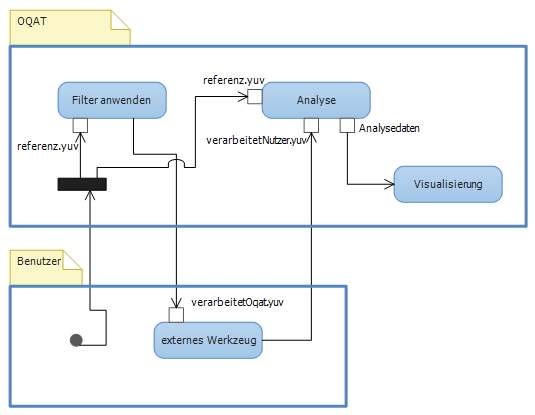
\includegraphics[scale=1]{bilder/einleitung.png}



